\chapter{Vergleich}
\label{ch:chapter05}
In diesem Kapitel werden die beiden Konzepte (Hierarchische Struktur und Minimalistisch) mittels eine Nutzwertanalyse betrachtet.
Diese sollen helfen zu betrachtet, welche der beiden Konzepte allgemein die vorher genannten Kriterien am meisten erfüllt.
Dabei werden die Ergebnisse der Prioritätsanalyse verwendet und basierend mit dem Erfolg, die das Konzept für das jeweilige Kriterium hat verrechnet und addiert.
Das Konzept mit einem höheren Wert erfüllt mehr die Kriterien als das andere.
Zum Abschluss wird die alternative racF begutachtet auf ihre Vor und Nachteile.

\section{Nutzwertanalyse}
\label{sec:chapter05:Nutz}
Für die Nutzwertanalyse müssen die jeweiligen \ac{TN} bestimmt werden.
Dies wird mittels \ac{Gf} mal der \ac{Zf} gemacht.
Daraus bildet sich der \ac{TN} und die Summe davon generiert den \ac{GN}.
Der höhere \ac{GN} zeigt, dass dieses Konzept einen höheren Nutzen hat.
Anzumerken dabei ist, dass wenn die \ac{GN} zu ähnlich sind, weitere Schritte vorgenommen werden sollen, um ein eindeutiges Rank zu erschaffen.
Für die \ac{Zf} wurde wieder ein vier Punktesystem ausgewählt.
Die Tabelle (\ref{fig:Ziel}) zeigt was die verschiedenen Zahlen bedeuten. \cite{BdIufH}
\begin{figure}[h!]
 \centering
 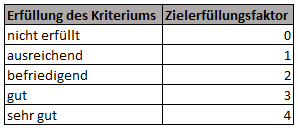
\includegraphics[width=1\textwidth]{gfx/Picture/Ziel.PNG}
 \caption{Die Zf Tabelle}
 \label{fig:Ziel}
\end{figure}
\newpage
\begin{figure}[h!]
 \centering
 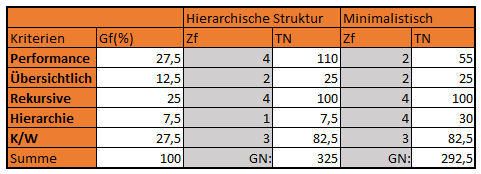
\includegraphics[width=1\textwidth]{gfx/Picture/Nutzwert.PNG}
 \caption{Nutzwertanalyse für die beiden Konzepte}
 \label{fig:Nutz}
\end{figure}

Wie man erkennen kann ist der \ac{GN} zwischen den beiden Faktoren bei lediglich $32,5$.
Da dieser unterschied zu gering ist, wird die Wermaßstäbe weiter verfeinert.
Dadurch ändert sich die Punkteskala und Tabelle wie folgt:
\begin{figure}[h!]
 \centering
 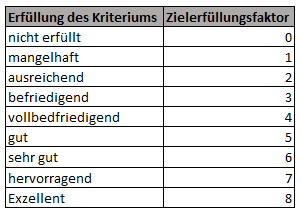
\includegraphics[width=1\textwidth]{gfx/Picture/Ziel2.PNG}
 \caption{Die Zf Tabelle}
 \label{fig:Ziel}
\end{figure}
\newpage
\begin{figure}[h!]
 \centering
 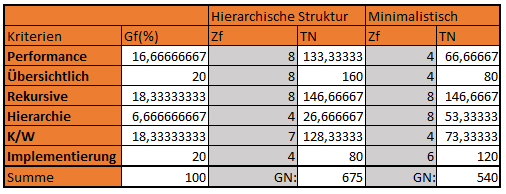
\includegraphics[width=1\textwidth]{gfx/Picture/Nutzwert2.PNG}
 \caption{Nutzwertanalyse für die beiden Konzepte}
 \label{fig:Nutz}
\end{figure}
Durch die Verfeinerung liegt der Unterschied zwischen den beiden Faktoren bei $82,5$.
Anhand der Verdopplung der Punkteskala hat sich der Unterschied fast verdreichfacht.
Wodurch das Konzept Hierarchische Struktur eindeutig im Rank an erste Stelle steht.

\section{Vor/Nachteile Hierarchische Struktur}
\label{sec:chapter05:Hierarchische}


\section{Vor/Nachteile Minimalistisch}
\label{sec:chapter05:Minimalistisch}
Donec gravida consequat arcu, et mollis tortor posuere vitae. Sed pharetra turpis a ante commodo accumsan. Suspendisse leo nulla, accumsan sit amet dapibus in, posuere eget turpis. Vivamus enim sapien, porta id placerat eget, laoreet sed massa. Class aptent taciti sociosqu ad litora torquent per conubia nostra, per inceptos himenaeos.

\section{Ablösung ins racF}
\label{sec:chapter05:racF}
Donec gravida consequat arcu, et mollis tortor posuere vitae. Sed pharetra turpis a ante commodo accumsan. Suspendisse leo nulla, accumsan sit amet dapibus in, posuere eget turpis. Vivamus enim sapien, porta id placerat eget, laoreet sed massa. Class aptent taciti sociosqu ad litora torquent per conubia nostra, per inceptos himenaeos.

